\documentclass[10pt]{article}
\usepackage[utf8]{inputenc}
\usepackage[T1]{fontenc}
\usepackage{amsmath}
\usepackage{amsfonts}
\usepackage{amssymb}
\usepackage[version=4]{mhchem}
\usepackage{stmaryrd}
\usepackage{graphicx}
\usepackage[export]{adjustbox}
\graphicspath{ {./images/} }

\title{SOLUTIONS FOR EXTRA ADMISSIONS TEST IN \\
 MATHEMATICS, COMPUTER SCIENCE AND JOINT SCHOOLS DECEMBER 2020 }

\author{}
\date{}


\begin{document}
\maketitle
A If the side length of the cube is $x$, then the distance between opposite corners is $x \sqrt{3}$. So here $x=2 / \sqrt{3}$ and the surface area is $6 x^{2}=8$

The answer is (c)

B Pair the terms for $(2 / 3)^{x}(4 / 5)^{x} \ldots(20 / 21)^{x}$. Each of these terms gets very small for large $x$, so the product gets close to zero.

The answer is (a)

C Must have

$$
\frac{240 x}{x^{2}+4}=360 n \pm 60
$$

for some whole number $n$. So

$$
4 x=(6 n \pm 1)\left(x^{2}+4\right)
$$

SO

$$
x^{2}-\frac{4}{6 n \pm 1} x+4=0
$$

Now if $n=0$ we get solutions $x=2$ and $x=-2$. If $n \neq 0$ then the discriminant of this quadratic $\frac{16}{(6 n \pm 1)^{2}}-16$ is negative, so no other solutions. So two solutions.

The answer is (c)

D The next few terms are

$$
y=2 x+3 x^{2}+5 x^{3}+7 x^{4}+11 x^{5}+13 x^{6}
$$

Only the $x^{5}$ term contributes to the value of the fifth derivative at $x=0$ (higher terms are zero because they include $x^{n-5}$ and lower powers give zero when differentiated five times). We get $5 \times 4 \times 3 \times 2 \times 1 \times 11=1320$

The answer is (e)

E There are some solutions with $x$ and $y$ both bigger than 1, with $x$ slightly larger than $y$. So not (a) or (c). If $-1<x<1$ then $x^{20}<1$, so $x^{20}-y^{20}<1$, since $y^{20}$ is positive. So no solutions in that range.

The answer is (d)

F Statement $P$ is equivalent to " $-1<x<1$ or $x<-2$ ". Statement $Q$ is equivalent to " $-1<$ $x<1$ ". So $Q$ implies $P$ but $P$ does not imply $Q$.

The answer is (b)

G We can use $S$ to make any positive integer. Then we can use $T$ on that positive integer to make any positive rational number with denominator a power of 2 . Or we can apply $T$ first, and repeatedly applying $T$ gives numbers down to -2 (almost). This is only consistent with option (e).

The answer is (e)

H $a_{n}=A^{2^{n}}$ so $b_{n}=2^{n} \log _{2} A$ which is a geometric progression, but not an arithmetic progression or a constant, because $\log _{2} A>0$.

The answer is (c)

I The other vertex of the triangle is at $(500,500 \sqrt{3})$ and the points inside are either in $x<500$, $x>500$, or down the middle $x=500$. Now $866<500 \sqrt{3}<867$ so there are 866 points down the middle. The total is therefore even. Imagine the parallelogram made by adding a triangle with vertices at $(1000,0)$ and $(500,500 \sqrt{3})$. There are approximately 866,000 points contained in these two triangles (866 rows of about 1000), so about 433,00 in each triangle. Only one option is both even and approximately 433,000.

The answer is $(\mathrm{d})$

$\mathbf{J}$ The region has reflectional symmetry in the $x$ axis and in the $y$-axis, so consider first the region in the quadrant where $x>0$ and $y>0$. In that region, the region is bounded by the parabolas $y=2-x^{2}$ from the second inequality, and $x=2-y^{2}$ from the last inequality. These parabolas meet at $(1,1)$. There is a line of symmetry in the line $y=x$, so we just need to find the area under the line $y=x$ between 0 and 1 (a triangle) and the area under the parabola $y=2-x^{2}$ between 1 and $\sqrt{2}$. Then we'll multiply this area by 8 .\\
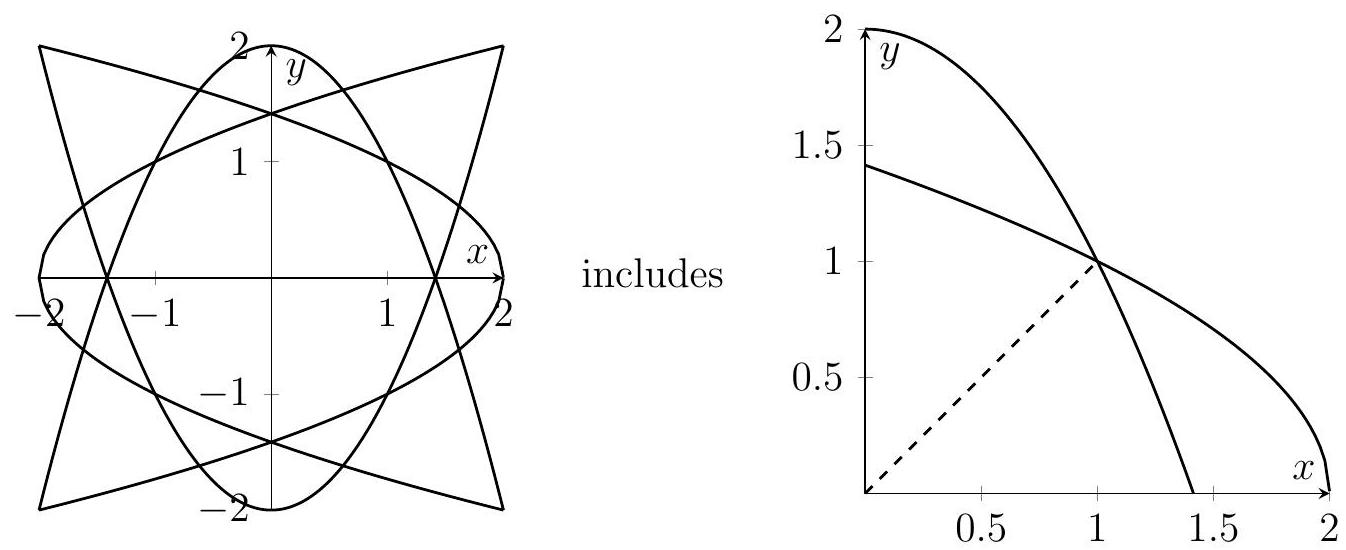
\includegraphics[max width=\textwidth, center]{2024_03_31_cff9f5ff88cecfd65df7g-2}

So we have

$$
8\left(\frac{1}{2}+\int_{1}^{\sqrt{2}} 2-x^{2} \mathrm{~d} x\right)=8\left(\frac{1}{2}+\left[2 x-\frac{x^{3}}{3}\right]_{1}^{\sqrt{2}}\right)=8\left(\frac{4}{3} \sqrt{2}-\frac{5}{3}+\frac{1}{2}\right)=\frac{4}{3}(8 \sqrt{2}-7)
$$

The answer is (d)


\end{document}